\section{Integration Experiments}
\label{text:experiments/integration}
In the following, the performance of the overall approach is evaluated. For comparison, several baselines have been re-implemented, that are frequently used in the field of crowd navigation: \ac{ORCA} \cite{vandenBerg2011}, \ac{RRT}$\star$ \cite{Karaman2011} and \ac{MCTS}. These baselines have been chosen, as they cover a broad field of existing trajectory planning methodologies, such as sampling-based, optimization-based or tree-search-based methods. \footnote{Section \ref{text:related/crowd_navigation} introduced the use of deep learning-based approaches in the field of crowd-navigation. Therefore, a state-of-the-art approach for socially-aware navigation using deep reinforcement learning, by Chen et alt. \cite{Chen2017}, should have been used as well. Unfortunately, it is neither open-source nor did the author reply to several of my requests.} The experiments have been conducted as described in Section \ref{text:experiments/setup}, using \ac{SGAN} \cite{Gupta2018} as an independent simulation environment and averaged several runs in a Monte-Carlo manner.

\subsection{Effect of Interactive Objective}
Figure \ref{img:show_case} illustrates the qualitative difference between the proposed approach and other planning approaches. Note that meanwhile, both algorithms can maintain some safety distance to the pedestrian. However, integrating the pedestrian prediction in the core of the optimization allows the solver to anticipate each pedestrian's future actions. While the path optimized by \ac{RRT}$\star$ (comp. Figure \ref{img:show_case}, right) cuts into the path of the green-colored pedestrian, the interactive-aware optimization chooses to stay behind the pedestrian, which is reasonable travel-time efficient but introduces a lot fewer disturbances on the surrounding pedestrians. 

\begin{figure}[!ht]
\begin{center}
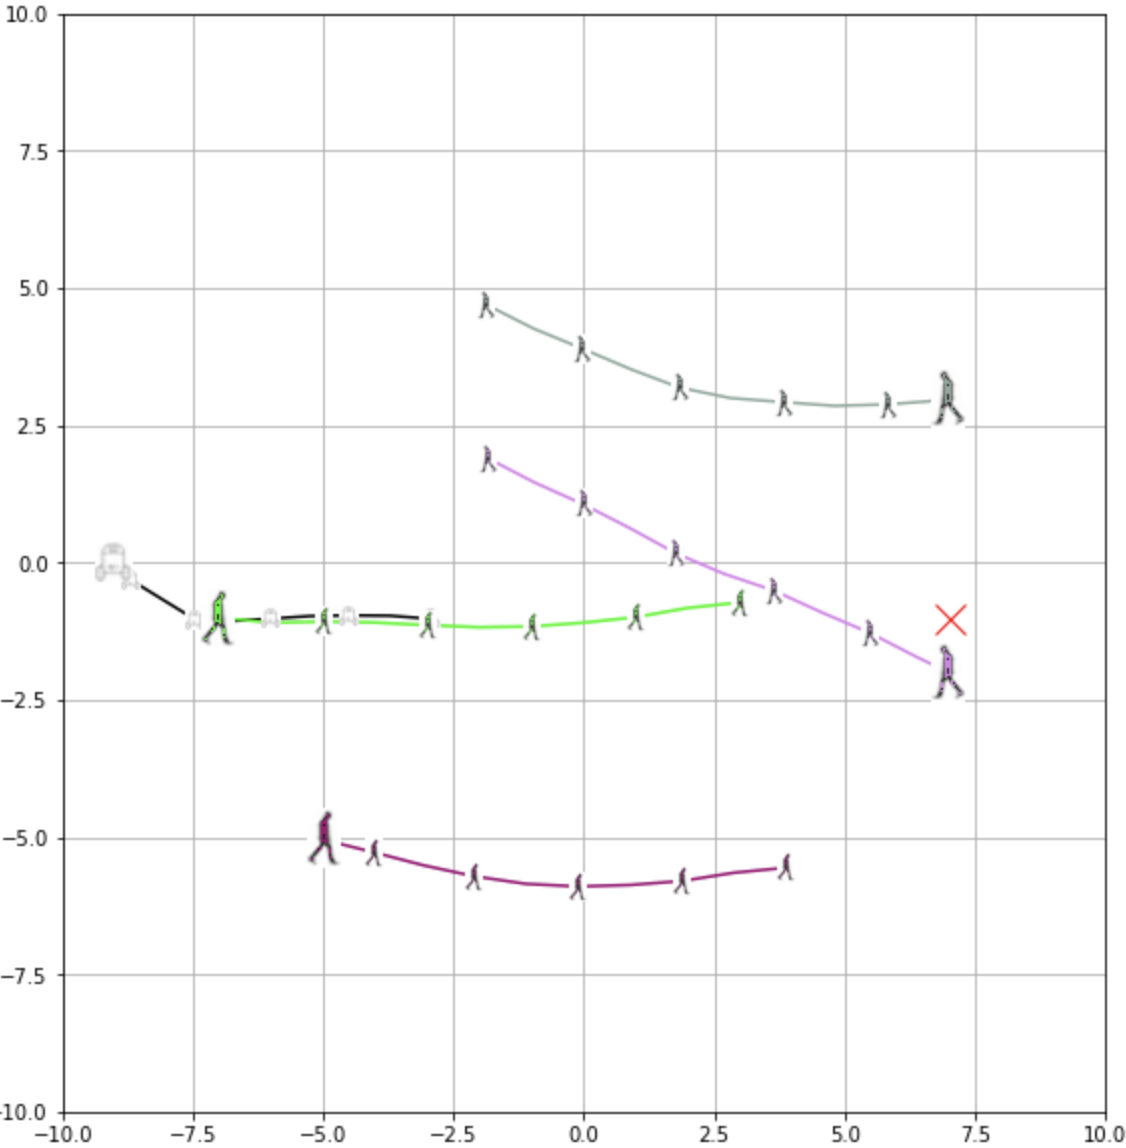
\includegraphics[width=0.45\textwidth]{images/show_case_ipopt.png}
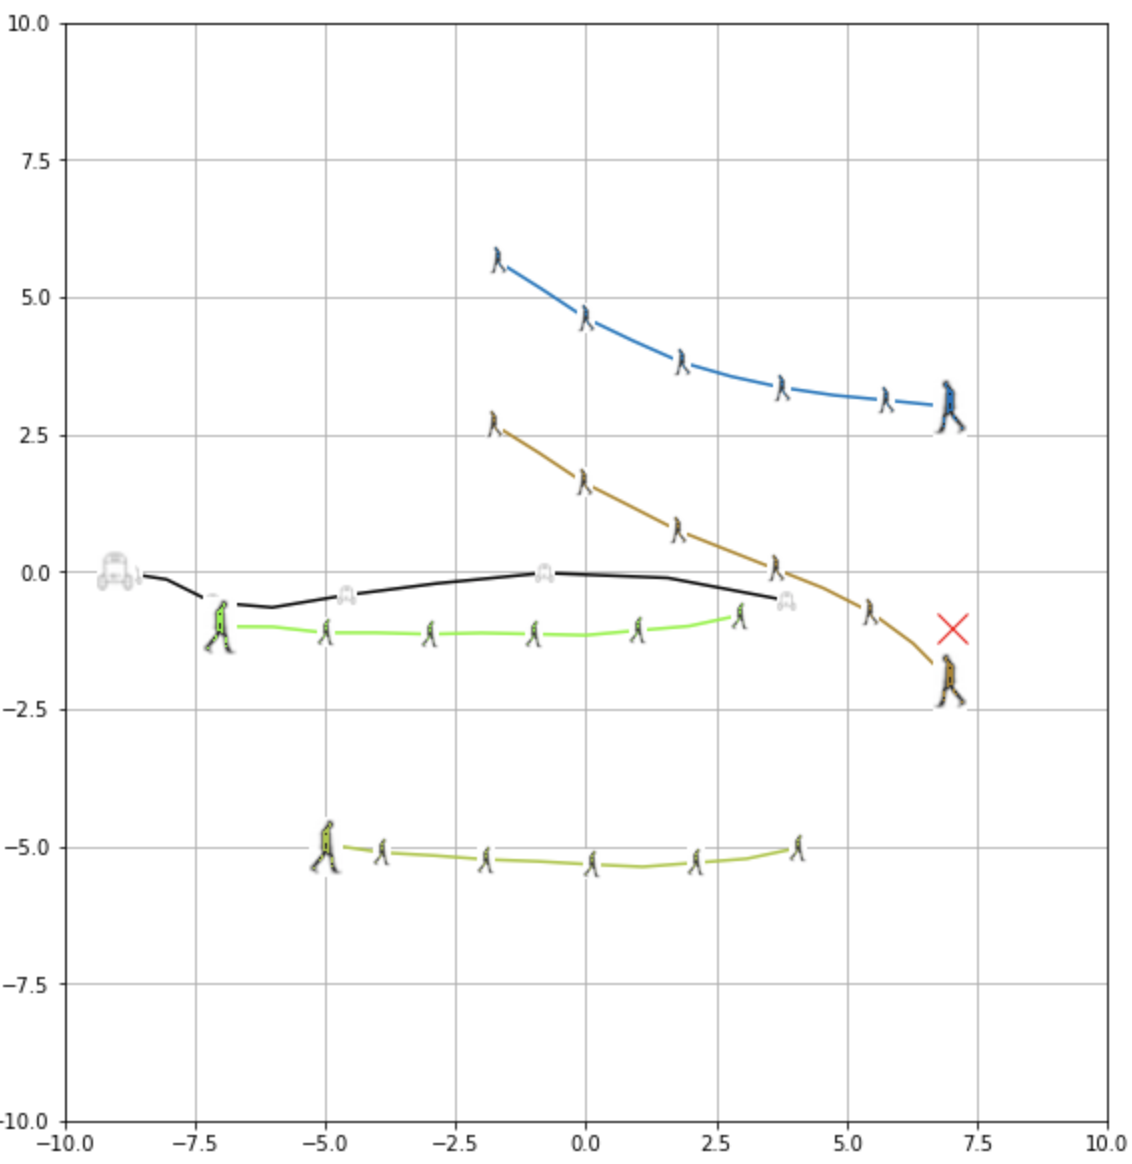
\includegraphics[width=0.45\textwidth]{images/show_case_rrt.png}
\end{center}
\caption{Exemplary comparison of generated trajectories by our approach (left) and \ac{RRT}$\star$ \cite{Karaman2011} (right)}
\label{img:show_case}
\end{figure}

\subsection{Baseline Performance}
The previously described qualitative benefits of the proposed approach can be underlined by quantitative results. The following experiments compare the quantitative results of the several planning algorithms in the presence of 2 to 10 pedestrians in the scene and randomly created. 

\begin{table}[!ht]
\begin{center}
\begin{tabular}{c|c|c|c|c|c|c|c}
\bf Method & \bf MPE[\%] & \bf RTD & \bf RCE[\%] & \bf ETT & \bf TGD & \bf MSD & \bf MSR \\
\hline
\ac{MCTS} & 104 & 0.77 & 125 & 0.69 & 0.511 & 4.64 & 0.67 \\
\hline
\ac{ORCA} & 102 & 0.70 & 143 & 0.0 & 0.35 & 3.68 & 0.028 \\
\hline
\ac{RRT}$\star$ & 105 & 193 & 1.18 & 0.0 & 0.68 & 3.38 & 0.29 \\
\hline
\rowcolor{our_color}
\project & 100 & 0.93 & 100 & 0.38 & 0.30 & 4.51 & 0.28
\end{tabular}
\end{center}
\caption{Quantitative comparison of approach to several baseline methods.}
\label{table:baselines}
\end{table}

As shown in Table \ref{table:baselines}, the proposed algorithm outperforms the baseline methods in nearly all metrics. Although \ac{ORCA} performs surprisingly well, causing the second lowest mean pedestrian effort \ac{MPE}, behind \project, it fails keep the same safety distance as the solution trajectories derived using the proposed formulation. In fact, \project manages to find a solution that trade-offs efficiency with safety and intervention regarding the pedestrians better than all of the other approaches.  

\subsection{Effect of number of Pedestrians}
Figure \ref{img:runtime_num_pedestrian} illustrates the average algorithm's runtime for one trajectory optimization, depending on the number of pedestrians. While the proposed approach ("ipopt") runs with about 2-3 Hz in case of many pedestrians, the runtime is notably sub-linearly depends on the number of pedestrians in the scene. This can be explained by the widespread usage of batching within the algorithm, including the prediction model, and the use of attention filters, which keep the number of considered pedestrians during optimization approximately constant.

\begin{figure}[!ht]
\begin{center}
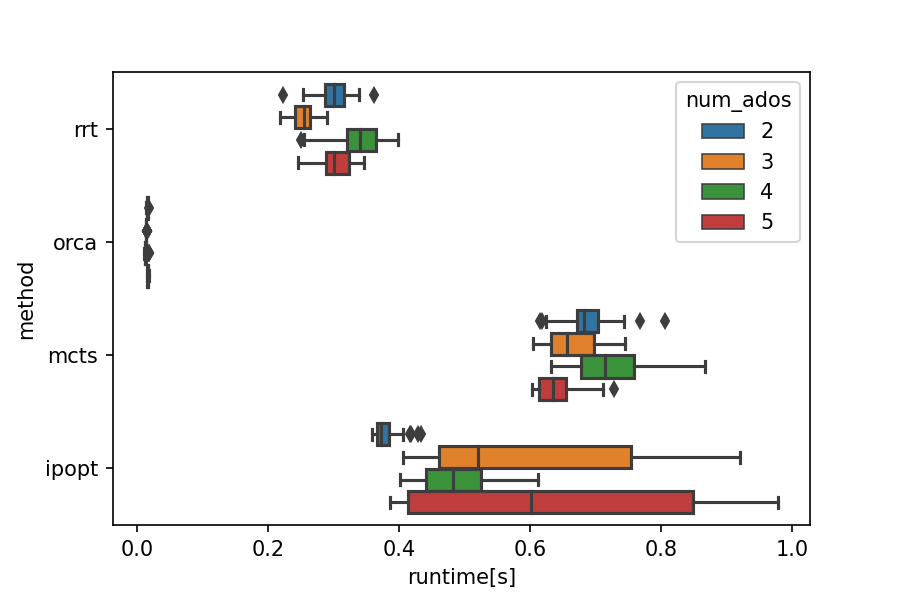
\includegraphics[width=\imgwidth]{images/runtime_peds.png}
\end{center}
\caption{Impact of number of pedestrians (ados) on algorithm runtime [s] (in logarithmic scale).}
\label{img:runtime_num_pedestrian}
\end{figure}

\subsection{Effect of Prediction Model}
The internal structure of the prediction model largely impacts, how a certain robot action is evaluated in terms of its interactive cost. Consequently, the optimized trajectories differ. However, it turns out that the qualitative properties of the solution trajectory are widely independent from the choice of prediction model, at least when the same simulation environment is being used. Figure \ref{img:effect_pred} illustrates this qualitative invariance, by comparing the solution trajectories of an optimization based on the Trajectron \cite{Ivanovic2018} (left) and the Potential Field model (right). As so, solution trajectory being derived using the latter environment tend to be single-agent focused. As described in Section \ref{text:exp_particles}, the Potential Field model neglects inter-pedestrian interactions and the robot does not impact a pedestrian's movement, if it is not in its field of view. Consequently, trajectories that are derived based on this environment, usually choose to follow behind the closest pedestrian. In contrast, the Trajectron models the effect each pedestrian has on all other agents in the scene. Thus, the robot chooses to stay behind the closest pedestrian, but in maximal distance to all other pedestrian. This has to pre-dominant reasons: Firstly, the pedestrians behavior is impacted by the robot, just due to its presence, and not limited by the pedestrian's field of view. And more importantly, secondly, intermediate effects are taken into account. Thus, when the robot has an impact on one pedestrian $k$, it might effect the others as well, since they might be effected implicitly by the change of action of $k$. 
\newline
However, although both solution trajectories in Figure \ref{img:effect_pred} differ in shape, they are qualitatively equal. Both robots choose to follow behind the closest pedestrian. This behavior can be observed over a wide range of different scenarios.

\begin{figure}[!ht]
\begin{center}
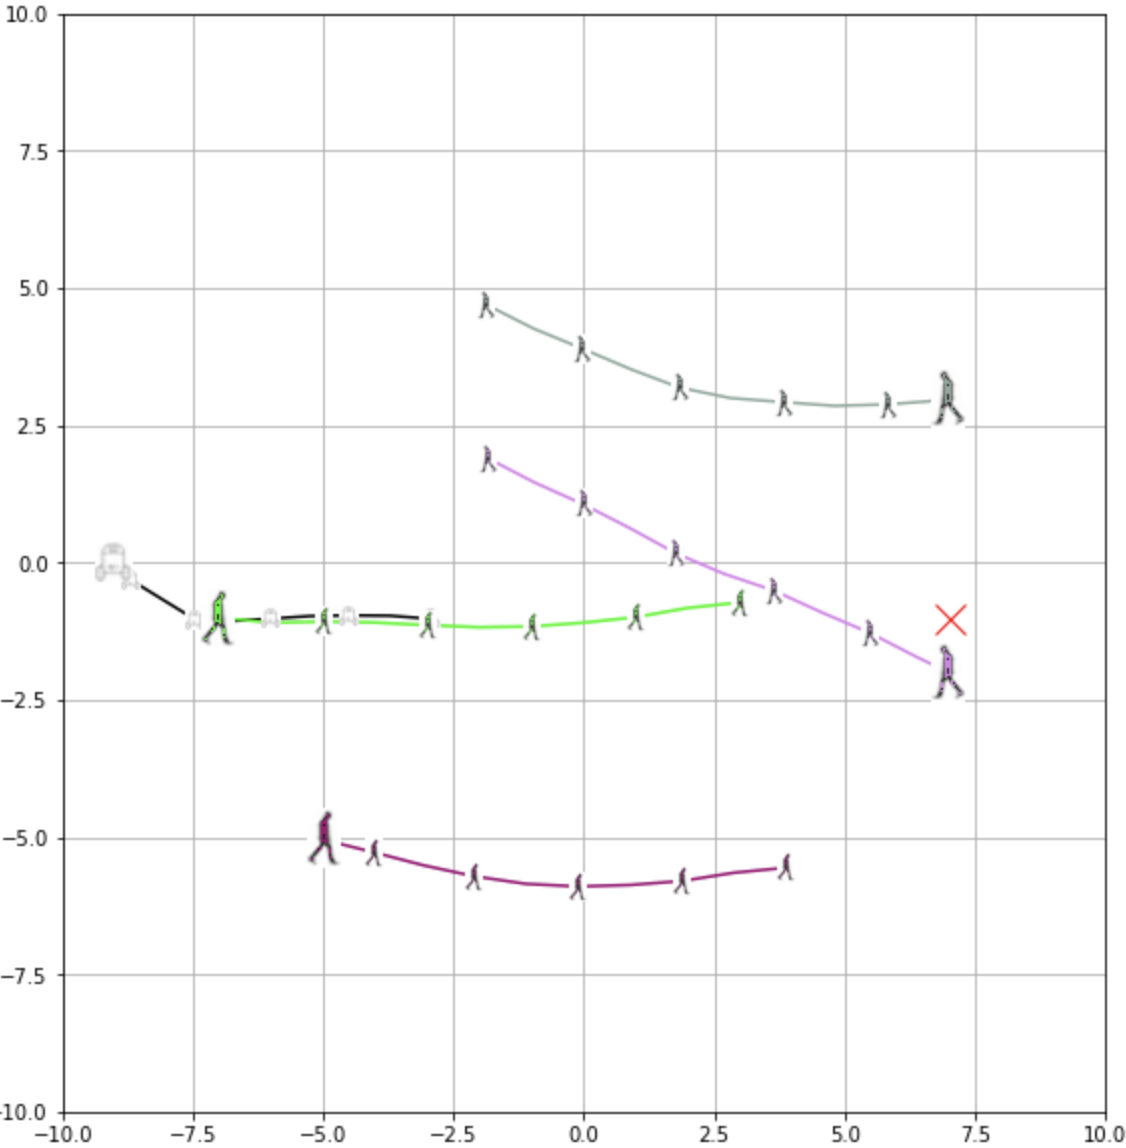
\includegraphics[width=0.45\textwidth]{images/show_case_ipopt.png}
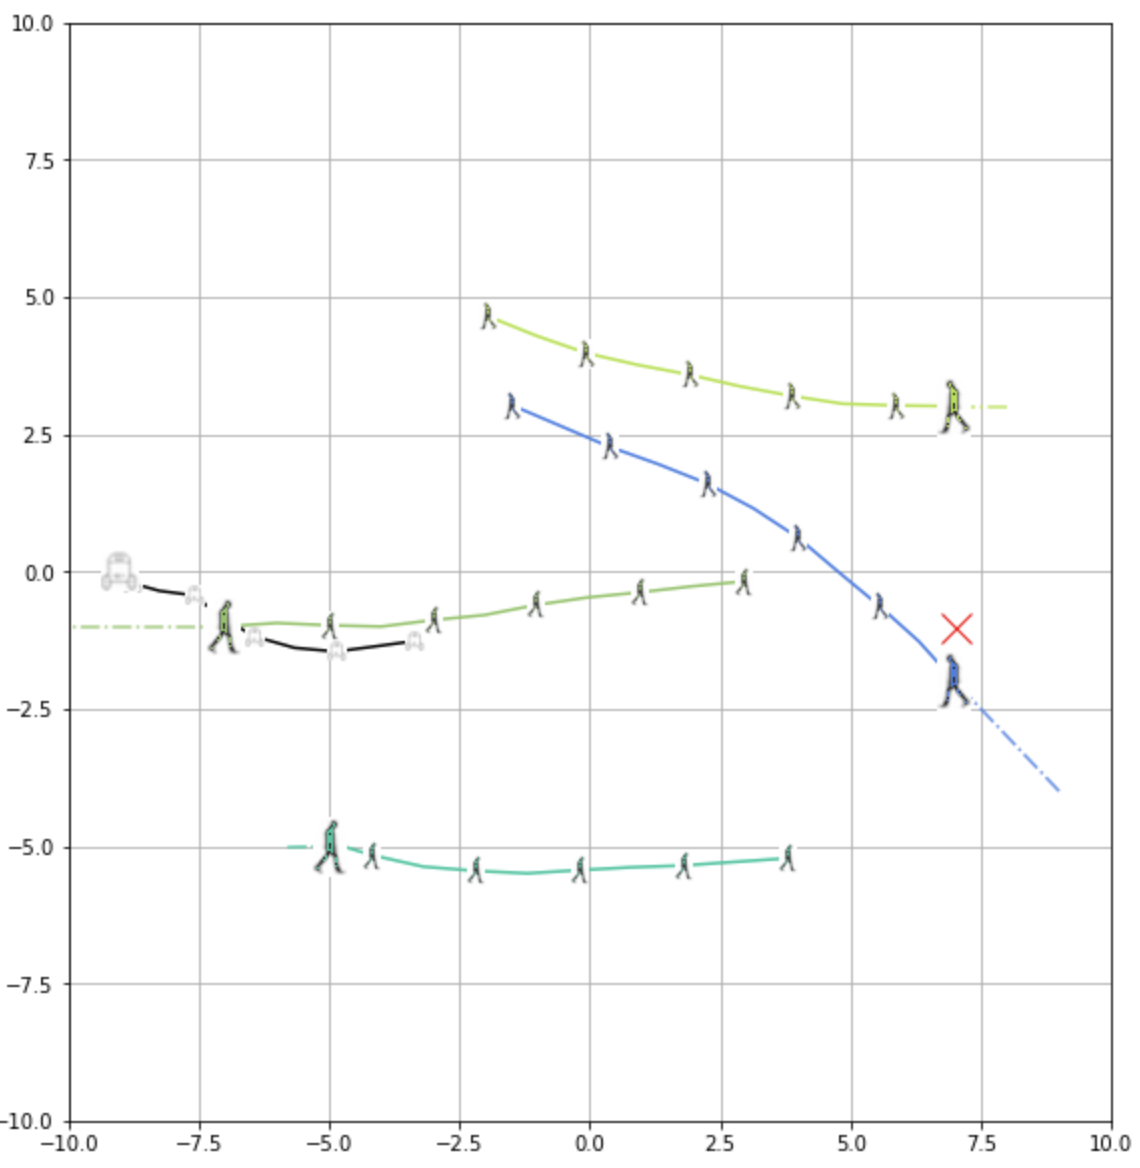
\includegraphics[width=0.45\textwidth]{images/impact_env_trajectron.png}
\end{center}
\caption{Exemplary comparison of generated trajectories by based on Potential Field model (left) and Trajectron \cite{Ivanovic2018} (right)}
\label{img:effect_pred}
\end{figure}